\section{Introduction}
\label{sec:intro}


% Do I want to say scalability?

% Goal
Storage systems is the foundational platform for modern Internet services. Ever increasing reliance on massive data sets has forced developers to move towards a new class of scalable storage systems known as NoSQL key-value stores (KV-store). Most distributed NoSQL KV-stores (e.g., Cassandra \cite{Cassandra}, Riak \cite{Riak}, Dynamo \cite{Dynamo}) support a flexible data schema and simple GET/PUT (or Read/Write) interface for reading and writing data items. 
The data items are replicated at multiple servers to provide high fault-tolerance and availability. 

One drawback of the replication-based approach is the high storage cost. Erasure coding (EC) has been integrated with other types of KV-store to reduce storage cost (e.g., Cocytus \cite{Cocytus2016} for in-memory KV-store  and Giza \cite{GIZA2017} for cross-datacenter KV-store).
This work is motivated by the following question: \textit{is it possible to use erasure coding in a NoSQL KV-store to reduce storage cost while maintaining strong consistency with moderate performance penalty?} We provide an affirmative answer by introducing \textbf{CassandrEAS (Cassandra + Erasure-coding Atomic Storage)}, a customized version of Cassandra \cite{Cassandra} with a new EC-based storage protocol that achieves \textit{atomicity} \cite{lamport}, a form of strong consistency.

\paragraph*{Cassandra}

% why Cassandra? why Strong consistency? what properties?
We chose to develop our system on top of Cassandra. Even though Cassandra was released in 2008, it is still one of the most used NoSQL KV-stores in industry. It is also an active open-source project (recent stable release in February 2020) \cite{DBEnginesCassandra}. Plus, its quorum-based replication \cite{pbs-vldb2012} shares similarly with other popular systems like Riak \cite{Riak} and Dynamo \cite{Dynamo}. For many big data applications, Cassandra offers a good balance of properties, e.g., high availability, scalability, and tunable consistency. Our system CassandrEAS provides similar guarantees in scalability and availability.%, because we aimed to integrate our protocol with Cassandra seamlessly (as will become clear later).


Cassandra offers tunable consistency guarantees, ranging from eventual consistency to strong consistency.
Popular storage systems in industry, such as Google Spanner \cite{Spanner} and CockroachDB \cite{cockroachDB}, are focusing on providing strong consistency. 
Inspired by the observation, this paper focuses on \textit{atomicity} \cite{lamport} (or linearizability \cite{herlihy1990linearizability}), one of the more popular forms of strong consistency, because atomicity is composable \cite{herlihy1990linearizability} and more intuitive for developing applications.

%Therefore, as the first step, CassandrEAS provides only atomicity.

Cassandra provides high availability and scalability using a quorum-based (or peer-to-peer) design.
It replicates data on multiple servers, and each server can serve any read/write request from clients 
using the practical quorum approach (or Dynamo-style quorum) \cite{pbs-vldb2012}. 
The approach does not use master node or consensus protocol to coordinate servers; hence, Cassandra has a high performance without a single point of failure. 
Cassandra's quorum-based design make it difficult to use prior EC-based solutions \cite{Cocytus2016,GIZA2017}, which either use a master-based design or consensus-based protocol.

\paragraph*{Main Contributions}

In this paper, we present our novel quorum-based storage protocol, One-Round Erasure coding Atomic Storage (\oreas). 
We implement \oreas{} into Cassandra \cite{Cassandra2010}, namely CassandrEAS.
More precisely, we replace Cassandra's replication mechanism by our EC-based protocol.
We try to make minimum modification to the original Cassandra codebase, and Cassandra users can call Cassandra's original read and write API directly \textit{without} knowing the details of the algorithm.\footnote{Our algorithm does not support transaction; hence, those transaction-related APIs are not supported. Note that Cassandra uses Paxos \cite{paxos} to support transactions, and this is why \oreas{} cannot be directly applied.} 
To the best of our knowledge, this is the first implementation in NoSQL KV-Store that uses erasure coding.\footnote{We will release our code on Github once the paper is accepted in hope that stimulate more discussion and evaluation on using erasure codes in similar systems.} 

Using \oreas{}, CassandrEAS also provides availability and scalability at a similar level of Cassandra, because both systems do not use master or consensus.
One interesting feature of \oreas{} is a \textit{tunable knob} that allows clients to choose the desired level of availability (i.e., the maximum number of tolerated server failures), storage cost, and the number of supported concurrent operations. If there are more server failures or more concurrent operations than the specified parameters, then CassandrEAS may return stale value or fail to serve client's request. A protocol for self-stabilization, reconfiguration, or recovery is left as an interesting future work.

For evaluation, we deploy CassandrEAS in Google Cloud Platform (GCP) and conduct extensive experiments using the Yahoo! Cloud Service Benchamarking (YCSB) workload generator \cite{YCSB:2010}. YCSB is a realistic tool used to benchmark many KV-stores.
%The implementation is discussed in Section \ref{s:implementation} and we present 
Our evaluation results in Section \ref{s:evaluation} indicate that CassandrEAS incurs moderate performance penalty, yet saves significant amount of storage space.

\paragraph*{Cassandra vs. CassandrEAS}
Table \ref{t:comparison} summarizes the comparison between Cassandra and CassandrEAS when storing one unit of data (i.e., data size is normalized to $1$). We do not count the size of meta-data such as timestamps. Erasure coding is more useful when dealing with larger data (say in terms of $100~B$s), so meta-data size is practically negligible. 
In our presentation, $n$ denotes the number of servers that store the data, $\delta$ represents \underline{the maximum number of writes concurrent with any read on} \underline{the \textit{same} key-value pair}, and $f$ is the maximum number of tolerated crash servers.
To make our formula compact, let $k = n-2f$. For Cassandra, we choose the majority quorum configuration.
% For Cassandra, we choose the quorum configuration. That is, both the read quorum and write quorum are of size $\frac{n}{2}+1$.

\begin{table}[h]
	\centering
	\begin{tabular}{ l|c|c}
		& Cassandra &  CassandrEAS  \\ \hline
		&&\\[-0.8em]
		Storage cost at each server & $1$ &  $\frac{1}{ \lceil\frac{k}{\delta+1}\rceil}$  \\
		&&\\[-0.8em]\hline
		%$~~~~~~~~~~~~~~~~~~~~~f$ 
		Fault-tolerance level $(f)$& $\frac{n}{2} - 1$     &  $\frac{n-k}{2}$  \\%\hline
		%Read (Write) cost & $1$ &  $\frac{n}{ \lceil\frac{\delta+1}{k}\rceil}$\\\hline
	\end{tabular}
	\caption{Cassandra (Quorum) vs. CassandrEAS}
	\label{t:comparison}
	%\caption{Comparison of key performance metrics among the three implementations of strong consistency in Cassandra. $\delta$
	%	is the maximum number of writes concurrent with any read.}
\end{table}

In practical systems, the number of concurrent writes \underline{on the \textit{same} KV-pair} is small in most cases, since each operation completes in the order of $100~ms$. If CassandrEAS with $n=9$ is configured to tolerate $f=2$ crashed servers, and support $\delta = 3$ concurrent writes. In this case, $k = 5$, so the data storage cost at each server becomes

\[
\frac{1}{ \lceil\frac{k}{\delta+1}\rceil} = \frac{1}{ \lceil\frac{5}{3+1}\rceil} = \frac{1}{2}
\]

In comparison, Cassandra's storage cost is $1$, as each server stores the original data. Hence, CassandrEAS saves $50 \%$ of storage space. If we have the configuration $n=7, f=1, \delta=1$, then $k=5$ and the storage cost of CassandrEAS is $\frac{1}{3}$, a $67\%$ reduction in storage space.



% Our work
%We propose two new EC-based storage algorithms: a two-round algorithm, \treasmod{} (Two-Round Erasure coding Atomic Storage), using logical timestamp, and a one-round algorithm, \oreas{} (One-Round Erasure coding Atomic Storage), using physical timestamp. Both algorithms tolerate network asynchrony and crash failures of any client and some fraction of servers, and achieve \textit{near-optimal storage cost}. Each algorithm achieves slightly different guarantees and performance.
%Similar to the design of vanilla Cassandra, if clocks drift significantly, then \oreas{} might violate strong consistency. On the contrary, \treasmod{} ensures strong consistency at all time, but suffers an extra round of delay due to the usage of logical timestamp.


%\begin{figure*}[!ht]
%	\begin{subfigure}[b]{\columnwidth}
%		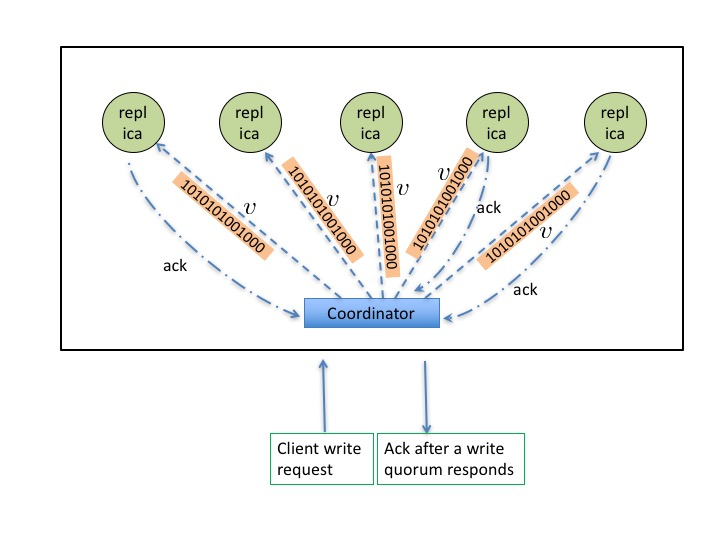
\includegraphics[width=\linewidth]{img/replication.jpg}
%		\caption{Cassandra stores the original value $v$.}
%		\label{fig:1}
%	\end{subfigure}
%	\hfill %%
%	\begin{subfigure}[b]{\columnwidth}
%		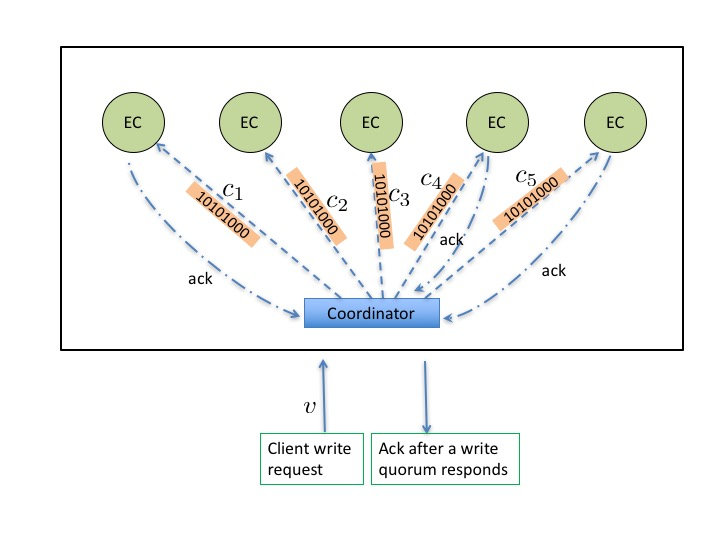
\includegraphics[width=\linewidth]{img/ec-code.jpg}
%		\caption{CassandrEAS only stores erasure-coded elements $c_i$'s.}
		%In TREAS and OREAS the erasure-coded elements of any value, e.g.,  $v$, is stored as  coded elements at separate servers.}
%		\label{fig:2}
%	\end{subfigure}
%	\caption{Illustration of Cassandra and CassandrEAS}
%\end{figure*}

% why EC?
% See motivaiton -- https://ipads.se.sjtu.edu.cn/_media/publications/cocytus_fast16.pdf
%\paragraph{Erasure Coding Storage Systems}
%\vspace*{3pt} \noindent \textbf{Erasure Coding Storage Systems}~~

\section{Preliminaries}

\paragraph*{Erasure Coding Storage Systems}
Erasure coding (EC) is a space-efficient solution for data storage. 
EC has been traditionally used with great success for storage cost reduction in \textit{write-once, read-many-times} data stores (e.g., \cite{rashmi_fast15, dimakis2011survey, sathiamoorthy, HuaSimXu_etal_azure}). Recently there is an increasing interest in using EC in update-many-times, read-many-times data stores. As observed in \cite{Cocytus2016,GIZA2017}, with the advancement of hardware, it is possible to perform encoding/decoding in a real-time fashion.
EC also has the potential to significantly reduce network bandwidth, as well as for system maintenance (such as repairing failed servers).
Therefore, both information theory and system research communities have investigated the usage of erasure coding to reduce various kind of costs, e.g., \cite{dimakis2010network, rashmi2016ec, tamo2014family}.

% Prior Work
Two recent systems Cocytus \cite{Cocytus2016} and Giza \cite{GIZA2017} studied the applicability of erasure coding in other types of KV-stores. 
Giza~\cite{GIZA2017}, Microsoft's proprietary storage,  is a Fast-Paxos-based  multi-version cross-data center strongly consistent object store used in Microsoft's OneDrive storage system. Giza servers store erasure-coded elements instead of the original data to significantly reduce storage cost. 
Cocytus~\cite{Cocytus2016} is a master-based in-memory KV-store that guarantees strong consistency and reduces storage cost using erasure coding.  For each key,  value is erasure coded and the coded elements are stored among a subset of servers. In addition, the master server maintains a full copy of the value to provide high availability for read operations. 
%Cocytus uses a master and Giza uses consensus to coordinate servers.
As elaborated above, Cassandra's quorum-based design does not fit well with consensus protocol or master-based design.
%Their system designs are completely different from Cassandra, a quorum-based system. 
Therefore, we have to design a new EC-based protocol for using erasure coding in Cassandra.


%Theory community also shows interest in using erasure coding.
%EC-based algorithms for strongly consistent storage are also an active area of research in theory community, e.g., \cite{CadambeLMM17, SODA2016, LDS2017}.  %SODA\cite{SODA2016} described an algorithm to achieve optimal storage cost; however, pays higher write communication cost. 
%None of these algorithms have been integrated or implemented real-world systems. It is not clear how to adapt them into practical systems.

\paragraph*{Erasure Codes}
In this paper, we consider the optimal erasure codes. In particular, we adopt an $[n, l]$  linear Maximum Distance Separable (MDS) code ~\cite{verapless_book} over a finite field $\mathbb{F}_q$ to encode and store the value $v$ among the $n$ servers. Value is referred to a specific version of the data in our context. An $[n, l]$ MDS code has the property that any $l$ out of the $n$ coded elements can be used to recover (or decode) the original value $v$. 
For encoding, $v$ is divided\footnote{In practice, $v$ can be viewed as a byte array, which is divided into many stripes based on the choice of the code, various stripes are individually encoded and stacked against each other. We omit details of represent-ability of $v$ by a sequence of symbols of $\mathbb{F}_q$, and the mechanism of data striping, since these are fairly standard in the coding theory literature.} into $l$ elements $v_1, v_2, \ldots, v_l$ with each element having  size $\frac{1}{l}$ (assuming size of $v$ is $1$). The encoder takes the $l$ elements as input and produces $n$ coded elements $c_1, c_2, \ldots, c_n$ as output, i.e., $[c_1, \ldots, c_n] = \Phi^{(n,l)}([v_1, \ldots, v_l])$, where $\Phi^{(n, l)}$ denotes the encoder. For ease of notation, we simply write $\Phi^{(n, l)}(v)$ to mean  $[c_1, \ldots, c_n]$. The vector $[c_1, \ldots, c_n]$ is  referred to as the codeword corresponding to the value $v$. Each coded element $c_i$ also has  size $\frac{1}{l}$. In our scheme, we store \textit{one coded element} per key-value pair at each server. 



\begin{algorithm*}[!ht]
	\begin{algorithmic}[2]
		{\footnotesize
			\begin{multicols}{2}
				
				\Statex /* at each reader  $r$ */
				\Operation{read}{} 
				%\State $wCounter\gets wCounter+1$
				\State $\tup{t_r, v} \gets \dagetdata{c}$
				\State $\daputdata{c}{ \tup{t_r,v}}$
				\State return $v$
				\EndOperation
				\Statex
				\Statex /* at each writer  $w$ */
				\Operation{write}{$v$} 
				%\State $wCounter\gets wCounter+1$
				%\State $t \gets $ machine time
				\State $t_w \gets (t, w)$ where $t$ is machine time at $w$
				\State $\daputdata{c}{\tup{t_w,v}}$
				\EndOperation
				
				\Statex
				\State /* helper functions for each $\pr_i$ */
				
				\Procedure{get-data}{}
				%	\State {\bf send} $(\text{{\sc query}},\rdr)$ to every server $s\in \bigcup_{cseq[i]}members(\qs_{cseq[i].conf})$
				\State {\bf send} $(\text{{\sc query-list}})$ to each  server $s$%\in \mathcal{S}$
				\State {\bf wait until}  receives $List_s$ from $\left\lceil \frac{n + k}{2}\right\rceil$ distinct servers%each server $s\in\srvSet_g$ s.t. $|\srvSet_g|=\left\lceil \frac{n + k}{2}\right\rceil$ 
				\State  $Tags_{*}^{\geq k} = $ set of tags that appears in  $k$ lists	\label{line:getdata:max:begin}
				\State  $Tags_{dec}^{\geq \ell} =$ tags appearing in $\ell$ lists with values
				\State  $t_{max}^{*} \leftarrow \max \{Tags_{*}^{\geq k} \}$; ~~~~~$t_{max}^{dec} \leftarrow \max \{ Tags_{dec}^{\geq \ell} \}$ \label{line:getdata:max:end}
				%\State  $t_{max}^{dec} \leftarrow \max \{ Tags_{dec}^{\geq \ell} \}$ \label{line:getdata:max:end}
				\If{ $t_{max}^{dec} \geq  t_{max}^{*}$} 
				\State  $v \leftarrow $ decode value for $t_{max}^{dec}$
				\EndIf
				%\State $List_M \triangleq \bigcup_{s \in \srvSet_g}  List_s$
				%$\State  $\forall t$, $List_M(t) \triangleq \{ (t, v): (t,v) \in List_M \}$  
				%\State $\forall t$, $T(t') \triangleq \{t: (t,v) \in List_M(t) \wedge t \geq t' \}$
				%\State $t_r \gets \max \{t : (t, *) \in List_M ~\wedge |List_M(t)| \geq k~\wedge |T(t)| \leq \delta \}$
				%\State $v_s\gets \text{decode from }  List_M(t_{r}))$
				\State {\bf return} $\tup{t^{dec}_{max},v}$
				\EndProcedure
				
				\Statex				
				
				\Procedure{put-data}{$\tup{\tg{},v})$}
				\State $\Coded = [(\tg{}, e_1), \ldots, (\tg{}, e_n)]$, $e_i = \Phi_i(v)$
				\State {\bf send} $(\text{{\sc write}}, \tup{\tg{},e_i})$ to each server $s_i$ %\in \mathcal{S}$
				\State {\bf wait until}  receives {\sc ack} from $\left\lceil \frac{n + k}{2}\right\rceil$ distinct servers
				\EndProcedure
				
			\end{multicols}
		}
	\end{algorithmic}	
	\caption{The steps for writers and readers in \oreas{}.}\label{alg:oreas-client}
\end{algorithm*}


\begin{algorithm*}[!ht]
	\begin{algorithmic}[2]
		{\footnotesize
			\begin{multicols}{2}
				\State{/* at each server $s_i$ */} %\in \mathcal{S}$}
				\State{\bf State variables:}%{ 										
				\Statex $List \subseteq  \mathcal{T} \times \mathcal{C}_s$, initially   $\{(t_0, \Phi_i(v_0))\}$
				
				\State
				\Receive{{\sc query-list}}{}%{$s_i,c_k$}
				\State Send $List$ to client $q$
				\EndReceive
				\State
				\Receive{{\sc put-data}, $\tup{\tg{},e_i}$}{}%{$s_i,c_k$}
				%{\color{blue}
				\State $\tg{max} = \max_{(t,c) \in List} \{t\}$
				
				\If{$\tg{} \geq \tg{max}$}   \label{line:treasmod:monotone:begin}
				\State /* Garbage collect old values */
				\State $List \gets List \backslash \{\tup{\tg{max},e_i}:  \tup{\tg{max},e_i} \in List\}$ 
				\State $List \gets List \cup \{\tup{\tg{},e_i}, \tup{\tg{max},\bot}\}$
				\Else
				\State $List \gets List \cup \{\tup{\tg{},\bot}\}$ \label{line:treasmod:monotone:end}
				\EndIf %}
				
				\State  Send {\sc ack} to client $q$
				\EndReceive
				
			\end{multicols}
		}
	\end{algorithmic}	
	\caption{The steps for server $s_i$ in  
		\oreas{}.}\label{alg:oreas-server}
\end{algorithm*}	


\paragraph*{Main Challenge}

The key challenge in an EC-based storage protocol that is compatible with quorum-based system is to handle concurrent operations.
To ensure high availability, the readers need to receive sufficient coded elements from the servers to be able to decode the version of the data that satisfies \textit{atomicity}. This issue becomes complicated in practice due to the following reasons: (i) there might be concurrent write operations that write different versions of the data simultaneously; (ii) servers and clients might crash so that the servers do not have enough coded element for a particular version; and (iii) messages might arrive in an arbitrary order due to the asynchrony assumption of the underlying network.
%If a read operation is concurrent with multiple write operations, then it is possible that the read is \textit{not} able to retrieve enough coded element to recover the original data. This situation becomes trickier with failures and asynchrony.

%There are two major ways of replicating data in KV-stores -- \emph{leader-based} or \emph{leaderless} strategy. Leader-based systems are often referred to as the primary-backup replication, with an appropriate consensus protocol like Paxos~\cite{PaxosSimple} or Raft~\cite{Raft} to elect a leader. Leaderless replication is mainly implemented based on quorum systems, and are used widely in NoSQL KV-stores.  The applicability of erasure coding in leader-based KV-stores has been recently explored in works like Cocytus \cite{Cocytus2016} and Giza \cite{GIZA2017}.  Our work is focused on using \textit{leaderless} strategy to provide strong consistency; hence, the technique is sufficiently different from prior leader-based storage systems. Moreover, we implement our algorithms in Cassandra, and show that CassandrEAS can handle typical NoSQL workload (using YCSB \cite{YCSB}) with low performance penalty.%, which was different from the in-memory \cite{Cocytus2016} and cross-datacenter systems \cite{GIZA2017}. 

%Cocytus~\cite{Cocytus2016} is a leader-based in-memory KV store that guarantees strong consistency. For each key, the ue is erasure coded and the coded elements are stored among a subset of servers. In addition, a primary server maintains a full copy of the value so as to provide high availability for read operations.  Giza~\cite{GIZA2017} is a leader-bsed cross-datacenter KV store that also guarantees strong consistency, and used in Microsoft's OneDrive storage system. Giza uses FAST-PAXOS (a variation of Paxos~\cite{PaxosSimple}) to elect the leader.
%The practicality of erasure-codes in Giza comes form the fact that an key-value pair is updated on average at most $4$ times during its life time.  

% Challenges
%\paragraph*{Challenges}
%\vspace*{3pt} \noindent \textbf{Challenges}~~
%On a high-level, erasure codes are more natural in leaderless systems than in leader-based systems. 

%%%%%%%%%%%%%%
%%%%%%% Maybe move Challenges to later??? %%%%%%%
%%%%%%%%%%%%%%

%\subsection{Challenges}
%Cassandra and other similar NoSQL KV-Stores  (e.g., \cite{Dynamo07,Riak}) use quorums to ensure strong consistency.  Specifically, they require the client (or a client proxy) to contact a group of servers. In replication-based protocols, the writer clients need to send \textit{identical} copies of data to all the servers in the quorum, which consumes unnecessary network bandwidth and storage space. The case of Cassandra is illustrated in Figure \ref{fig:1}. On the contrary, in EC-based protocols, clients only send or receive \textit{coded elements} from servers. This substantially reduces not only the storage overhead but also the communication overhead.

%The main challenge of using EC in quorum systems is efficient handling of read operations. %concurrent with write operations. To ensure high availability, the reader clients need to receive sufficient coded elements from the servers to be able to decode the original data (and complete the read operation). This issue becomes complicated in practice due to the following reasons: (i) there might be concurrent write operations, (ii) servers and clients might crash, and (iii) messages might arrive in an arbitrary order due to the asynchrony assumption of the underlying network.

\commentOut{++++++++++
\subsection{Main Contributions}

\paragraph*{Contributions: Protocol Design}
We propose a new EC-based distributed storage algorithm -- One-Round Erasure coding Atomic Storage (\oreas{}). Our algorithm tolerates network asynchrony and crash failures of any client and some fraction of servers, and achieve \textit{near-optimal storage cost}.
%Similar to the design of vanilla Cassandra, if clocks drift significantly, then \oreas{} might violate strong consistency. On the contrary, \treasmod{} ensures strong consistency at all time, but suffers an extra round of delay due to the usage of logical timestamp.
%We propose a new EC-based storage scheme. If we use logical timestamps for each operation, then it requires two rounds to complete an operation, namely \treasmod. In this case, strong consistency is guaranteed at all time. On the other hand, if we use physical timestamps (i.e., machine time), then it only requires one round to complete an operation, namely \oreas. Similar to the replication-based protocol in Cassandra, \oreas{} might violate strong consistency if clocks at servers drift significantly.
\oreas{} has two benefits listed below. Let $\delta$ represent the maximum number of writes concurrent with any read.
\begin{itemize}
	\item The storage cost at each server is $\frac{B}{ \lceil\frac{\delta+1}{k}\rceil}$ bits for storing $B$-bit data. The new storage scheme is at least as efficient as the common EC-based protocols where each server stores codeword symbols for $\delta$ versions, e.g., \cite{ARES:ICDCS:2019}. Furthermore, for certain parameters of $\delta,k$, the new scheme can be up to twice as storage-efficient. For example, if we use an $[n = 5, k = 3]$ MDS code, the storage cost is simply  $1.67$ per unit of data, instead of $5$ as in the case of vanilla Cassandra.
	
	%\item An $[n, k]$ erasure code splits the value $v$ of size $1$ unit into $k$ elements, each of size $\frac{1}{k}$ units, creates $n$ {\em coded elements}, and stores one coded element per server. The size of each coded element is also $\frac{1}{k}$ units, and thus the total storage cost across the $n$ servers is $\frac{n}{k}$ units. For example, if we use an $[n = 5, k = 3]$ MDS code, the storage cost is simply  $1.67$ per unit of data, instead of $5$ as in the case of replication-based algorithms, such as ABD.
	
	
%	$B/\lceil \frac{l}{\delta}\rceil$ bits. Since $\frac{\delta}{l} \geq 1/\lceil \frac{l}{\delta}\rceil,$ the new storage scheme is at least as efficient as the common EC-based protocols where each server stores codeword symbols for $\delta$ versions, e.g., \cite{ARES:ICDCS:2019}. Furthermore, for certain parameters of $\delta,l$, the new scheme can be up to twice as storage-efficient. %as previous EC-based protocols. 
	
	\item In the new scheme, as in most replication-based approaches (such as the well-known replication-based algorithm by Attiya, Bar-Noy, and Dolev~\cite{ABD96} and Dynamo-style quorum systems \cite{Cassandra2010,Dynamo07,pbs-vldb2012}),  each server stores \underline{exactly one version of the data.} This is contrast to previous EC-based protocols (e.g., \cite{CadambeLMM14}) where $\delta$ versions of the data are stored at the server. 
\end{itemize}

%(which we refer to as ABD)

\paragraph*{Contributions: System}

We implement \treasmod{} and \oreas{} into Cassandra \cite{Cassandra2010}, namely CassandrEAS.
We pick Cassandra to be our base system due to its popularity and wide applications.
Cassandra adopts a practical partial quorum approach (or Dynamo-style quorum) \cite{pbs-vldb2012} for replicating data.
We replace its replication mechanism by our new EC-based protocols.
We try to make minimum modification to the original Cassandra codebase, and Cassandra users can call Cassandra's original read and write API directly \textit{without} knowing the details of the algorithm.\footnote{Our algorithm does not support transaction; hence, those transaction-related APIs are not supported.} 
To the best of our knowledge, this is the first implementation in NoSQL KV-Store that uses erasure coding.\footnote{We will release our code on Github once the paper is accepted in hope that stimulate more discussion and evaluation on using erasure codes in similar systems.} 

For evaluation, we deploy CassandrEAS in Google Cloud Platform (GCP) and conduct extensive experiments using the Yahoo! Cloud Service Benchamarking (YCSB) workload generator \cite{YCSB:2010}. YCSB is a realistic tool used to benchmark many KV-stores.
The implementation is discussed in Section \ref{s:implementation} and we present evaluation results in Section \ref{s:evaluation}.

++++++++++++=}





% prior work. We can talk about key-value systems that are completely different and does not use quorums (so we don't have to worry about comparing) or large systems like Giza, a proprietary system. What do you think we take a motivation as below.

% our contribution



% Kishori's guideline
%a)  is it possible to even use EC code based key-value in Cassandra, which is a super popular key-value, store to reduce storage cost? 
%b) But wait a minute, Cassandra wants strong consistency, which is not so easy with failure, asynchrony and EC,  however, it uses replication and quorum for now but might be possible to use EC with quorums
%c) Thankfully, we created a simple algorithm with might be possible to put into Cassandra.
%d) With lots of pain we managed to implement it in Cassandra, and got some interesting results.
%e) Let me describe the results to you now




\section{One-Round Erasure coding Atomic Storage}
%A particular form of the  strong consistency we are interested, i.e., atomicity, is composability. 
In this section, we describe our EC-based storage protocol -- One-Round Erasure coding Atomic Storage (\oreas).
One desirable property of atomicity \cite{lamport} (or linearizability \cite{herlihy1990linearizability}) is composability \cite{herlihy1990linearizability}.
That is, a collection of atomic storage units used together in an arbitrary way still satisfy atomicity. Note that some other forms of strong consistency might not have such a property. This is also why we are interested in providing atomicity. Due to composability, we describe \oreasSpace in terms of a single key-value pair (KV-pair), i.e., the key field is omitted in our discussion.
Our implementation supports multiple clients accessing multiple KV-pairs.
In our evaluation, we test CassandrEAS with multiple keys.
%We assume the value of our KV-pair is encoded, using a $MDS[n, k]$, into $n$ coded elements $c_1, c_2, \cdots c_n$ where each $c_i$ is stored at server $s_i$.  
%We provide two protocols: \treas{} and \oreas{}, whose pros and cons are described in later paragraphs.  
Due to space constraint, we briefly describe our protocol at a high-level along with the pseudo-code. %Figure \ref{fig:2} provides an illustration. 
Most technical details (including proofs) are presented in the accompanied technical report.\footnote{Our report is not currently available on web due to anonymous clause. If the paper is accepted, we will upload it to arxiv.}
The pseudo-code for readers and writers is presented in Algorithm \ref{alg:oreas-client}, and pseudo-code for servers is in Algorithm \ref{alg:oreas-server}.




%\vspace*{3pt}
%\noindent\textbf{TREAS}~~
%\subsection{OREAS}

\paragraph*{Meta-data} \oreas{} uses tags, where  a tag $\tg{}$ is defined as a pair $(z, w)$ such that $w$ is an unique ID of the writer, and $z$ is the local machine time (when the writer issues a specific write operation). 
%Note that in Cassandra, the writer corresponds to the user proxy (i.e., a coordinator); hence, the local machine time is synchronized.
Every pair of tags can be compared in the lexicographical order. It is reasonable to use machine time in our context, since the ``client'' is a proxy server (or a coordinator), which has a synchronized clock with other servers. In fact, Cassandra uses machine time to identify new values as well. For the case that time synchronization is difficult, we have another protocol, called \treas{}, which uses a logical timestamp to replace the machine time. 
For brevity, we focus on \oreasSpace in this paper.
%The detail are presented in our technical report.

\paragraph*{Write Operation} Suppose $v$ is the value that the writer intends to update the KV-pair with. The writer (or writer proxy) encodes $v$ to coded elements $c_1, c_2, \cdots c_n$, along with tag $\tg{}$, and sends the corresponding element to each server. Every server that receives a coded element
stores the coded element in its $List$ and performs garbage collection (i.e., replacing elements with smaller tags or storing a pair with $\perp$ value field). Finally,
% garbages collect the store coded element in its $List$ if the  corresponding tag is smaller than $t_{max}$ and 
it sends an acknowledgment message back to the writer. Once the writer receives acknowledgments from $\lceil\frac{n+k}{2}\rceil$  servers, it completes the write operation.

\paragraph*{Read Operation} The reader (or reader proxy) requests all servers for the lists of values. Upon receiving the request,  a server sends its local variable $List$ containing $(t, c_i)$ or $(t, \bot)$ to the reader.  
%\red{There are at most $\delta$ of them in the list???}. \blue{Each server stores in $List$  all the tags that it receives in the execution; even if the coded element corresponding to a tag $t$ is garbage collected, the server stores a tuple of the form $(t, \bot)$ } 
Once the reader receives responses from  $\lceil\frac{n+k}{2}\rceil$ of the servers, it decodes the value $v$ corresponding to the tag $t_{max}$. 
Our protocol ensures that as long as the number of crashed servers is  $\leq f$ and the number of concurrent writes is $\leq \delta$, a value is always decodable, and atomicity is satisfied.
Next the reader computes the coded elements of $v$, and together with the servers executes the steps as in the write operation (i.e., write-back phase), and then completes the read operation.  %Note that we have argued analytically that as long as the system does not experience concurrency more than $\delta$, the reads will always decode correctly. 


\paragraph*{Correctness}
We prove our protocols satisfy strong consistency (atomicity) in our technical report. We also develop a consistency checker based on the approach specified in \cite{Lynch1996} to ensure that our implementation also provides this guarantee. Validating strong consistency requires precise clock synchronization across all servers, since it needs to use global clock to ordering operations and events. This is impossible to achieve in a distributed system where clock drift is inevitable. To circumvent this, we deploy our CassandrEAS servers on a single machine and use Mininet \cite{MininetWebsite} to simulate the underlying network communication. Our checker then uses the machine time as the global clock. We collect multiple traces of 20,000 operations under different configurations with potentially machine failures. The checker verifies that all traces we tested satisfy strong consistency.
%so that every process observers the same clock running in the VM. 

%Our checker gathers meta-data regarding an execution of operations, such as start and end times, and timestamps.
%, and this data includes start and end times of all the operations, as well as other parameters like logical timestamps used by the protocol. 
%The checker logic is based on the conditions appearing in Lemma 13.16~\cite{Lynch1996}, which provide a set of sufficient conditions for guaranteeing strong consistency. The checker validates strong consistency property for ever KV-pair individually for the execution under consideration. We collect multiple traces of 20,000 operations under different configurations with potentially machine failures. The checker verifies that all traces we tested satisfy strong consistency.


%\paragraph{OREAS} %The implementation of OREAS is as follows, where instead of the logical tags we rely on physical timestamps, i.e., machine time at the coordinator.

%\emph{read} The read operation of OREAS is similar to that of TREAS. 

%\emph{write} The primary difference between TREAS and OREAS is that TREAS uses logical time stamp (or tag) where as OREAS uses the physical time at the write client  as the largest tag.  As a result, in OREAS th write operation simply involves using the current physical time to tag the  coded elements to a set of $  $ servers. Therefore, it does not need any round to recover the largest tag at the server 
%\vspace*{3pt}
%\noindent\textbf{OREAS}~~
%\subsection{OREAS}
%Instead of logical timestamp (tags), \oreas{} relies on physical timestamps, i.e., machine time at the coordinator. The advantage of using logical timestamp is that strong consistency is guaranteed even in the presence of clock drift and absence of synchronized clocks among the various servers.  The downside is that it requires, as in \treas{}, an additional communication round in order to gather the largest tag, which increases latency. On the other hand, in  \oreas{}, the strong consistency guarantee is reliant on correctly synchronized clocks; however, write operations complete in one round.
%In our setting every server stores only one, corresponding to the most recent tag received, coded element of dimension $\lceil\frac{k}{\delta+1}\rceil$. Therefore, there is no explicit garbage collection required.

%\paragraph{Storage cost}
%\vspace*{3pt}
%\noindent\textbf{Storage cost}~~
\paragraph*{Storage Cost}
In \oreas{}, erasure coding is used, and each server stores a list of all the tags that it has received so far. If a server receives the coded element corresponding to a tag newer than the current KV-pair with timestamp $t$, the server would update the current KV-pairs to the form $(t, \bot)$. The key feature that is different from other EC-based algorithms (e.g., \cite{dimakis2010network, rashmi2016ec, tamo2014family,GIZA2017,CadambeLMM17, SODA2016, LDS2017,Cocytus2016}) is that each server stores \emph{exactly one coded element} in $List$ and the rest of the elements in $List$ are of 
the form $(t', \bot)$, where $t'$ is some tag or timestamps that were garbage collected and $\bot$ is a place holder for null data. The  cost of storing one value of unit size at each server is hence $\frac{1}{ \lceil\frac{k}{\delta+1}\rceil}$. Recall that $\delta$ is
the maximum number of writes concurrent with any read operation, and $k = n-2f$.



\section{CassandrEAS}
\label{s:CassandrEAS}

\subsection{Implementation}

We share our implementation experience here in hope to lower the barrier of implementing other replication- or EC-based protocols in Cassandra in the future.
We have two main goals in our implementation: (i)
make minimum modification to the original Cassandra codebase;%, e.g., using Cassandra's original way of communication between servers; 
%For example, we try not to introduce new complicate data structure; and 
 (ii)
allow Cassandra users to use our implementation \textit{without} knowing the details of \oreas. That is, users can use the same Cassandra API in our system. 
The implementation turns out to be a difficult task because we are constrained to using only Cassandra's internal tools and data structures for communication and coordination. We spent enormous amount of time to decompose and understand Cassandra's internal logic because the codebase is not well documented and often provide poor comments. 
The version of Cassandra (version 3.11) that we used to develop contains around 57,000 LoC in Java. 
We also implemented the algorithm \treas, which uses logical timestamp to deal with loosely synchronized clock.
Our implementation of both algorithms consists of around 2,000 LoC.

%\vspace{3pt}
%\noindent\textbf{Data Model}~~
%%%%%%%%%%%%%%%%%%%%%%%%%%%%%%%%%% DO I NEED THIS??? %%%%%%%%%%%%%%%%%%%%%%%%%%%%%%%%%%
%\paragraph*{Data Model}
%Cassandra adopts the column-family data model, which provides a richer functionalities than a simple read-write object (KV-pair).  At a high level, Cassandra's data structure can be viewed as a table, where each row corresponds to data sharing the same key. CassandrEAS uses a row to store one KV-pair. Recall that the maximum number of writes concurrent with any read is denoted by $\delta$.  We use $2+2\delta$ columns for each row: key, value (a place holder for original data), and additional $2\delta$ columns for each version of the write. For each version, we use one column for timestamp (either physical or logical timestamp), and the other for the corresponding coded element. The reason that we need the value column is that it allows Cassandra to return the original data (decoded element) to the client. That column does \textit{not} store any data in storage. Each server only stores one coded element. The rest would be $\perp$ as discussed previously.

%Also since Erasure Encoding needs to ensure order, we assign an individual id number to the individual node. In our Schema, node\_ID starts at 1 and ends at the number of servers.


%In Cassandra, user first contacts the coordinator (or client proxy), and the coordinator follows the replication algorithm to read or write the data on the behalf of the Cassandra user. In other words, coordinator \textit{is} the client with respect to the replication algorithm. Therefore, in the presentation below, we will use coordinator and client interchangeably. In Cassandra's design (more specifically, the consistent hashing protocol), each server is a coordinator handling a certain set of keys.
%\vspace{3pt}
%\noindent\textbf{Technical Details}~~
\paragraph*{Technical Details}
We mainly modify the following two files in the Cassandra codebase. 
In Cassandra's terminology, ``mutation'' is essentially a write operation that modifies the internal state of the servers.
(i) \textit{StorageProxy.java} is where the coordinator server handles the user's read or write operation. Specifically,
\textsc{mutate} function handles Cassandra user's write operation whereas \textsc{fetchRows} function handles user's read operation. 
The size of read/write quorums is also specified in this file; and (ii) \textit{MutationVerbHandler.java} where each server's database engine handles incoming write requests from the coordinator.
Specifically, \textsc{doVerb} function applies the mutation onto local storage.

One major challenge we encountered is that Cassandra does \textit{not} provide an easy way to fetch users' requests and modify their mutations.
We have to figure out a way to construct a new mutation when we need to add new fields such as timestamp and coded elements.
Recall that we do not want to introduce new data structure, so we choose to use Cassandra's column family data model (i.e., an ordered collection of rows) to store the List variable at each server.
%\vspace{3pt}
%\noindent\textbf{Erasure Coding}~~
%\subsection{Erasure Coding}
CassandrEAS uses BackBlaze Reed-Solomon Code.\footnote{https://github.com/Backblaze/JavaReedSolomon}  These details are presented in our technical report.


\begin{figure*}[!ht]
	\begin{subfigure}[b]{0.32\textwidth}
		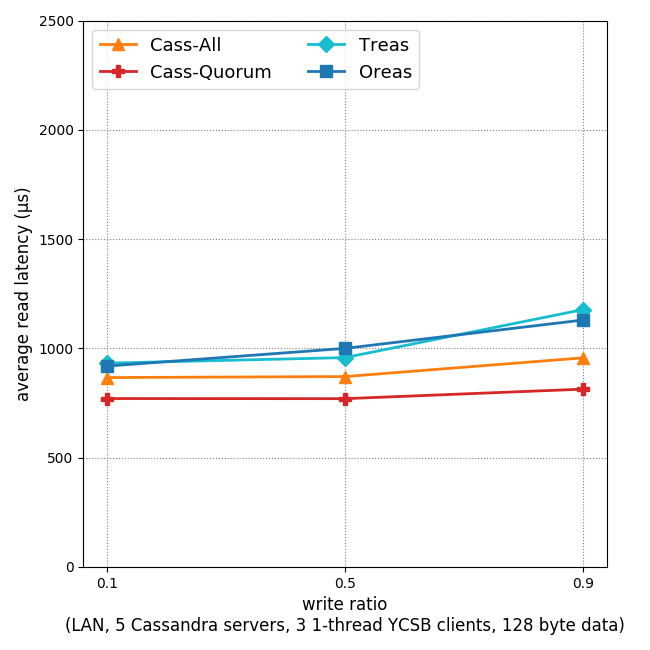
\includegraphics[width=0.9\linewidth]{img/LAN_7_latency,_vary_write,_5_svrs,_average_read.png}
		\caption{average read latency vs. write ratio}
		\label{fig:latency-read-ratio-avg}
	\end{subfigure}
	\hfill %%
	\begin{subfigure}[b]{0.32\textwidth}
		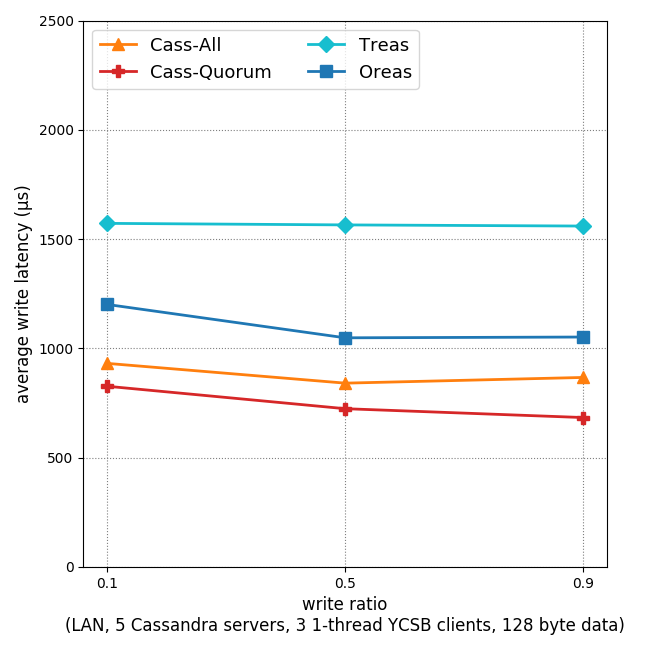
\includegraphics[width=0.9\linewidth]{img/LAN_9_latency,_vary_write,_5_svrs,_average_write.png}
		\caption{average write latency vs. write ratio}
		\label{fig:latency-write-ratio-avg}
	\end{subfigure}  
	\hfill %%
	\begin{subfigure}[b]{0.32\textwidth}
		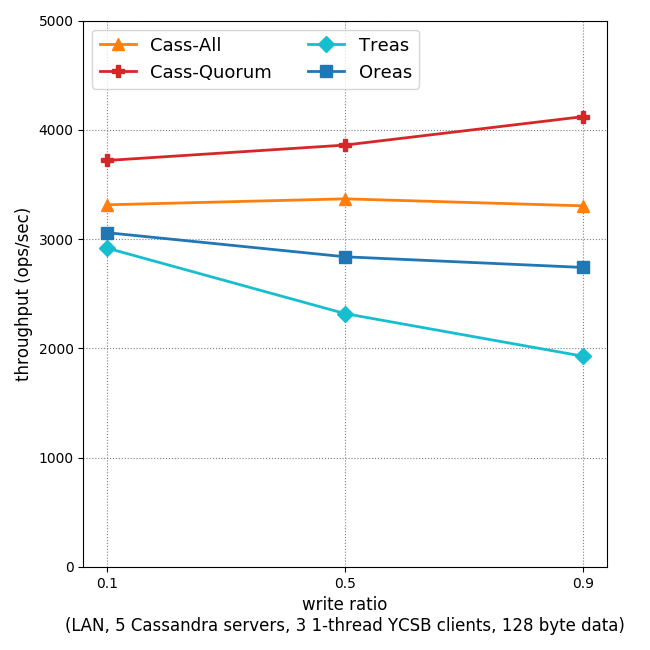
\includegraphics[width=0.9\linewidth]{img/LAN_6_throughput,_vary_write,_5_svrs.png}
		\caption{throughput vs. write ratio}
		\label{fig:throughput-ratio}
	\end{subfigure}

	\begin{subfigure}[b]{0.32\textwidth}
		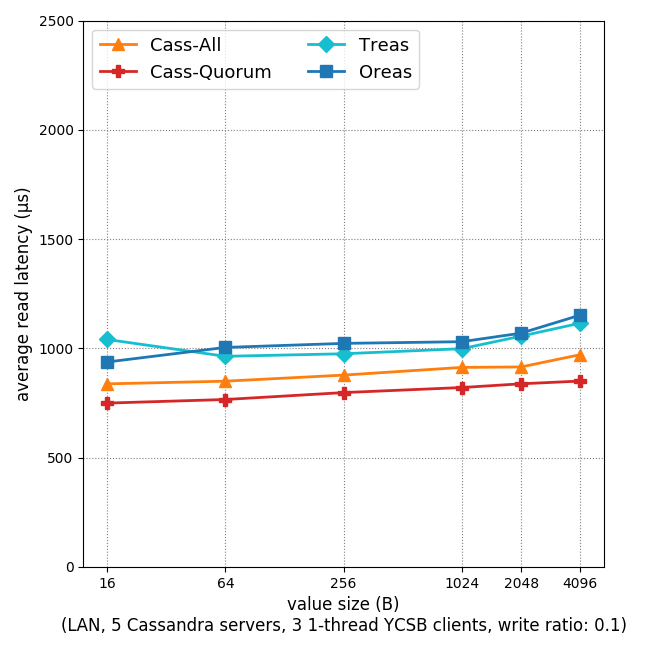
\includegraphics[width=0.9\linewidth]{img/LAN_12_latency,_vary_size,_5_svrs,_average_read.png}
		\caption{avg read latency vs. data size}
		\label{fig:latency-read-size-avg}
	\end{subfigure}    	
	\hfill
	\begin{subfigure}[b]{0.32\textwidth}
		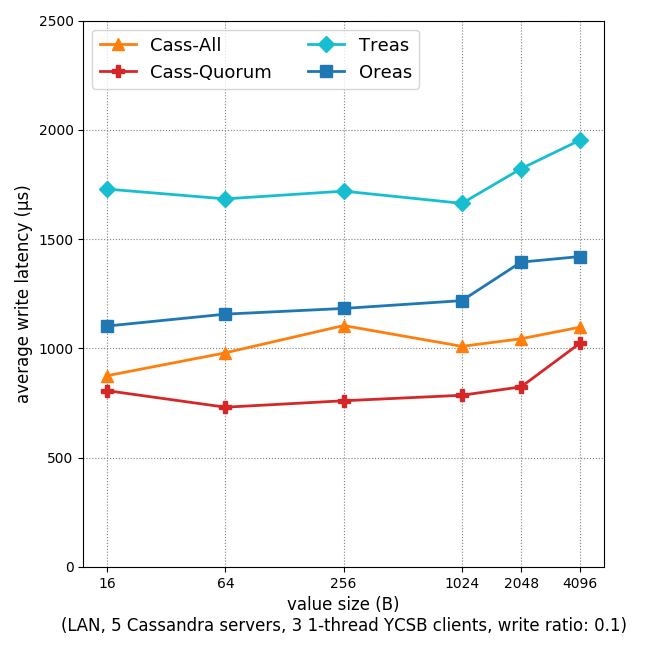
\includegraphics[width=0.9\linewidth]{img/LAN_14_latency,_vary_size,_5_svrs,_average_write.png}
		\caption{avg write latency vs. data size}
		\label{fig:latency-write-size-avg}
	\end{subfigure}    	
	\hfill %%	
	\begin{subfigure}[b]{0.32\textwidth}
		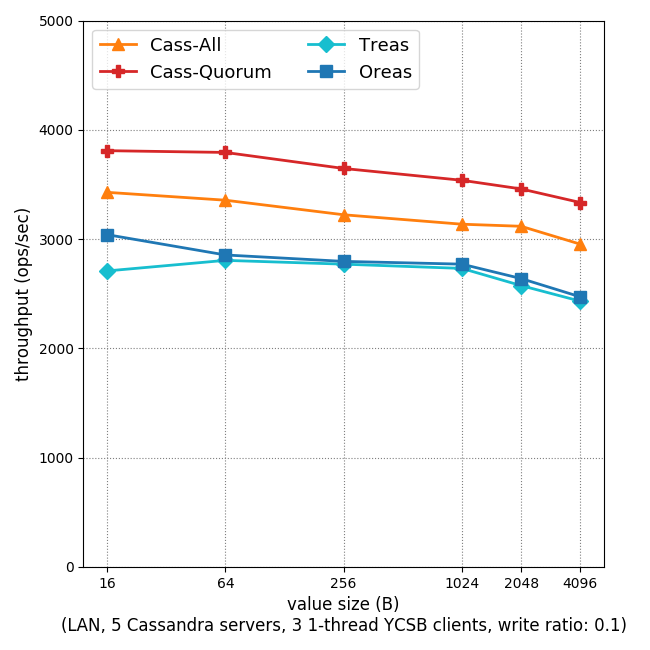
\includegraphics[width=0.9\linewidth]{img/LAN_11_throughput,_vary_size,_5_svrs.png}
		\caption{throughput vs. data size}
		\label{fig:throughput-size}
	\end{subfigure}    
	%	\hfill DON"T SHOW THIS ==> need to argue about inconsistent result for the %%%
	%	\begin{subfigure}[b]{0.3\textwidth}
	%		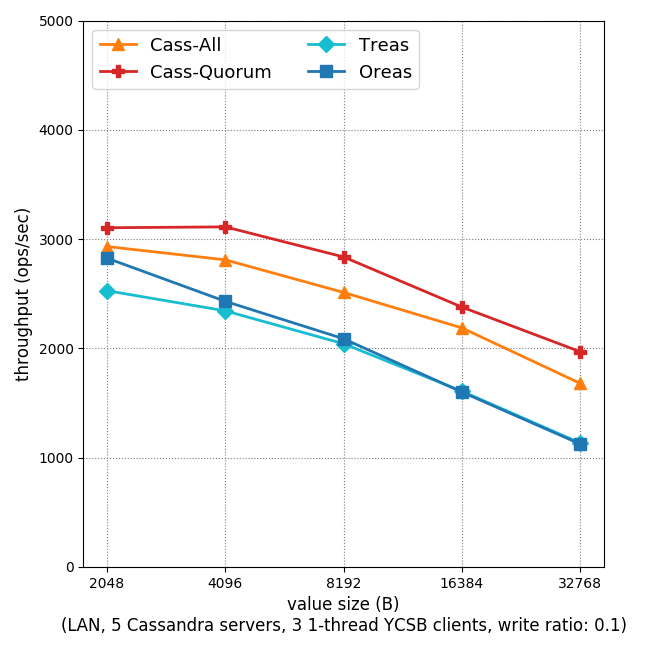
\includegraphics[width=0.9\linewidth]{img/LAN_16_throughput,_vary_size,_5_svrs.png}
	%		\caption{throughput vs. large data size}
	%		\label{fig:throughput-size-large}
	%	\end{subfigure}    	
	\caption{Comparison of latency and throughput of different configurations}\label{fig:evaluation}
\end{figure*}

%\section{CassandrEAS: Evaluation}
\subsection{Evaluation}
\label{s:evaluation}

We evaluate the performance of CassandrEAS by comparing it to the vanilla Cassandra (version 3.11). 
Cassandra-All requires the coordinator to hear from every server, whereas Cassandra-Quorum only requires to hear from a majority quorum of servers.

%and Cass-ABD. Cass-ABD replaced Cassandra's replication protocol with ABD \cite{ABD96}, which is a storage algorithm based on logical timestamps.
%We present the highlights of our evaluation results below:

%\begin{itemize}
%	\item \red{What should be here?}
%\end{itemize}

%\subsection{Experimental Setup}

%\paragraph{Cluster Configuration}
%\vspace*{3pt}
%\noindent\textbf{Cluster Configuration}~~
\paragraph*{Cluster Configuration and Workload}
We use the Google Cloud Platform (GCP) as our testing platform.
Each virtual machine (VM) is equipped with 4 virtual CPUs, 16 GB memory, and hosting Ubuntu 14.04 LTS.
All VMs are located in datacenter us-east1-c (South Carolina).
VMs use internal IP’s for communication.
The average RTT between any two VMs is around $0.3$ ms (based on issuing command for 30 seconds), and TCP bandwidth measured by Iperf is around $7.5$ Gbits/sec. %We use ping to estimate RTT.
For most of evaluation, our cluster consists of 5 VMs, and 3 YCSB single-threaded clients. Thus, $\delta = 3$.

%\paragraph{Workload}
%\vspace{3pt}
%\noindent\textbf{Workload}~~
%\subsection{Workload}
We use Yahoo! Cloud Serving Benchmark (YCSB) to generate realistic workload. We first insert a total of 30,000 KV-pairs, and each user performs 100,000 read or write operations. Recall that we have 3 YCSB clients, so we have 300,000 operations in total. We report the aggregated throughput, i.e., the sum of total operations per second across three YCSB clients. %We use the ``default Workload A'' provided by YCSB, whose operations follow Zipfian distribution.

%We use the Yahoo! Cloud Serving Benchmark (YCSB) \cite{YCSB} for evaluation. We did not choose Cassandra's own stress test tool, because it does not provide a straightforward way to disable Batch operation. Furthermore, it uses auto-generated data for all columns predefined.
%All of our YCSB workloads are modified from the ``default Workload A'' -- read-update workload. That is, YCSB first issues all-key insert before benchmarking, and we only benchmark on the read/update performances. 

%\vspace{3pt}
%\noindent\textbf{Performance}~~
\paragraph*{Performance}
Figure \ref{fig:evaluation} presents our evaluation results in different configurations.
Figures \ref{fig:latency-read-ratio-avg} to \ref{fig:throughput-ratio} show latency and throughput under different write ratio with data size equal to $128 B$. Read latency is comparable across all four algorithms. \treas{} has poor write latency due to the usage of logical timestamps, which requires an extra round-trip. \oreas{} has moderate penalty in write latency. 
Throughput is comparable in the case of write ratio $0.1$, a common case in NoSQL KV-stores.
Figures \ref{fig:latency-read-size-avg} to \ref{fig:throughput-size} show latency and throughput under different data size with write ratio $0.1$. We only show average latency, as 95 percentile has the same pattern.  Figure \ref{fig:throughput-size} demonstrates that CassandrEAS suffers moderate penalty on throughput.

%If we compare Figures \ref{fig:throughput-size} and \ref{fig:throughput-ratio}, then we see small discrepancy between throughput numbers. These two sets of experiments were conducted on different days. We have observed that performance can vary by around $10\%$ in different days with GCP. However, we are fairly confident that our evaluation methodology eliminates potential biases and noises. 

%Our evaluation results demonstrate that CassandrEAS provides latency and  throughput comparable to Cassandra in some cases. The average and 95 percentile latency numbers for reads and writes are shown in Fig~\ref{fig:evaluation} . The plots for throughput of operations under various value sizes and read to write frequency ratios further substantiates that there is no blocking operations due various workload properties. We obtained similar availablity and throughput results when we introduce server crashes. 

%\paragraph{Availability and Fault-tolerance}
%\vspace{3pt}
%\noindent\textbf{Aavailability and Fault-tolerance}~~
\paragraph*{Availability, Fault-tolerance, and Scalability}
CassandrEAS is highly available, fault-tolerant, and scalable, because its core is based on Cassandra.
It can continue serving client's operations as long as the conditions specified by $f$ and $\delta$ are satisfied.
We have tested our system with 7 servers and 1 crashed server, and observed minimal disruption on throughput (ranging from $0.1\%$ to $2.5\%$ decrease). We also observed that each YCSB client's throughput decreased a bit right after a server crashed, and later came back to normal throughput (compared with a cluster without any fault). Finally, we also tested clusters with 7, 9, and 11 servers. The throughput of \oreasSpace is in the range of $77 - 80 \%$ of Cassandra's. This demonstrates that CassandrEAS' performance is also scalable, i.e., the throughput increases when $n$ increases.
%some data with n=7, delta=3, 16B, w/r = 0.1
%name     throughput
%Treas-f=0 2682.11
%Treas-f=1 2610.55
%Oreas-f=0 2702.34
%Oreas-f=1 2697.6
%Indeed, the throughput just decreased a little bit. I also observed that the throughput at each YCSB client decreases 100-200 ops/sec for less than 10 seconds then comes back as normal.


\section{Discussion Topics}

\begin{itemize}
    \item \textit{Future work}: The current implementation of CassandrEAS only supports KV-pairs, whereas Cassandra supports column family data model. We would like to discuss potential trade-offs and solutions to support various data model. Another interesting direction is the mechanism to support efficient geo-replication. Since each server stores a smaller amount of data, with proper design, the EC-based solution might be more efficient than the replication-based protocol (under certain workloads).

    \item \textit{Importance/Applicability}: Some researchers warned us that it is \textit{not} reasonable to sacrifice performance for storage space. However, in our views, there are certainly needs for reducing storage, as the amount of data is growing exponentially. Moreover, if we want to apply distributed storage systems on top of smaller machines (e.g., edge servers or even Internet-of-Things), then storage-efficient solutions are certainly appealing. We would love to learn new ideas on use cases and interesting trade-offs to explore.
    
    \item \textit{Feasibility/Evaluation}: We only performed evaluation through YCSB. However, the use cases for EC-based storage systems might be very different from the normal cloud storage. It will be interesting to learn what workload is suitable for evaluating this type of systems.
    
    \item \textit{Open theoretical problems}: Right now, CassandrEAS only supports read/write operations, but not transactions, whereas Cocytus \cite{Cocytus2016} and Giza \cite{GIZA2017} supports transactions. Lightweight EC-based transaction mechanism is one interesting open problem. Another category of open problems is self-stabilization, reconfiguration, and recovery protocols discussed earlier.
    
    \item \textit{Open engineering problems}: In our implementation of CassandrEAS, we did not introduce any optimization. The reason is that as the first step, we want to make a minimal modification to Cassandra's core functions to demonstrate feasibility. For further optimization, there are two possibilities: modifying the database engine and cache protocol so that it is more friendly to coded elements, and introducing more efficient data structure to store coded elements.
    
    \item \textit{Limitations/Opportunity}: \oreas{} provides a knob to user to tune the performance and desired guarantees. Real-world systems also provide many different knobs. Unfortunately, knobs are usually difficult to tune in practice, because the trade-off is not always clear. Is it reasonable to expose the knob to users? What is the best way to help users (for selecting the most appropriate knob)? 
\end{itemize}